\chapter{Android & Wi-Fi direct}

Android è un sistema operativo per dispositivi mobili sviluppato da Google, basato su kernel Linux.
La sua progettazione è principalmente per smartphone e tablet, ma possiede anche interfacce utente specializzate per televisori (Android TV), automobili (Android  Auto), orologi da polso (Android Wear), occhiali (Google Glass) ecc… .
Essendo basato su kernel Linux possiede una licenza (Licenza Apache) che consente di modificare e distribuire liberamente il codice sorgente. 
Inoltre, tutte le applicazioni sono scritte soprattutto in linguaggio di programmazione Java.
Ogni release del sistema possiede un nome simbolico ed è rigorosamente dato seguendo l'ordine alfabetico, ed inoltre ogni nome corrisponde ad una golosità presente nel mondo, qua di seguito la lista delle varie versioni: la 1.5 venne chiamata Cupcake, la 1.6 Donut, la 2.1 Eclair, la 2.2 Froyo, la 2.3 Gingerbread, la 3.0 Honeycomb, la 4.0 Ice Cream Sandwich, la 4.1 Jelly Bean, la 4.4 Kit Kat. 
Attualmente l’ultima versione del sistema operativo è la 5.0, chiamata Lollipop.


\section{API}

\subsection{Architettura Android}

L'architettura di Android si suddivide in vari livelli (o layer), ognuno dei quali offre un servizio a quello superiore.
Vediamoli nel dettaglio:

\begin{center}
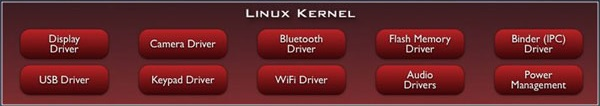
\includegraphics[width=1\textwidth]{imgs/Linux Kernel.jpg}
\captionof{figure}{Livello più basso dell'architettura Android}\label{linux_kernel_img}%
\end{center}

Nella figura \ref{linux_kernel_img} viene rappresentato il livello più basso di tale architettura, che contiene il kernel di Linux.
Inoltre, comprende anche vari driver per la gestione delle diverse periferiche: dallo schermo alla tastiera, dalla scheda di rete Wi-Fi all'alimentazione.

\begin{center}
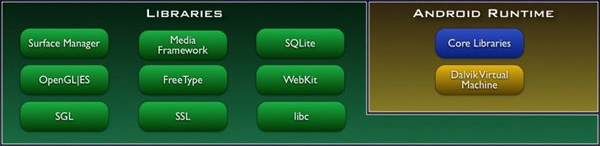
\includegraphics[width=1\textwidth]{imgs/Librerie.jpg}
\captionof{figure}{Tale livello rappresenta il cuore di Android}\label{librerie_img}%
\end{center}

Salendo invece al terzo livello, troviamo tutte le Librerie native che sono state svillupate nel linguaggio C/C++ figura \ref{librerie_img}.
Tutte insieme tali librerie rappresentano il cuore di Android, qui di seguito alcuni componenti delle librerie nello specifico: Surface Manager, che gestisce la componente grafica
Media Framework, implicata nella gestione dei codec audio e video
La libreria SSL che gestisce il Secure Socket Layer.

\begin{center}
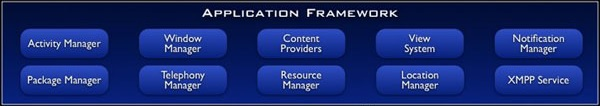
\includegraphics[width=1\textwidth]{imgs/Applicazioni_Framework.jpg}
\captionof{figure}{Livello composto da una serie di componenti API}\label{applicazioni_framework_img}%
\end{center}

Salendo ancora al quarto livello troviamo l'Application Framework figura \ref{applicazioni_framework_img}, formato da un insieme di API che svolgono specifici compiti:
Activity Manager, fondamentale in quanto è responsabile dell'interazione tra applicazione e utente.
Window Manager per la gestione delle finestre delle varie applicazioni.
Package Manager responsabile della gestione del ciclo di vita delle applicazioni.

\begin{center}
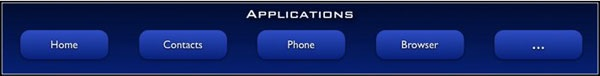
\includegraphics[width=1\textwidth]{imgs/Applicazioni.jpg}
\captionof{figure}{Ultimo livello che racchiude le applicazioni vere e proprie}\label{applicazioni_img}%
\end{center}

Arrivati all'ultimo livello, troviamo le Applicazioni vere e proprie che utilizzano i livelli sottostanti per essere eseguite figura \ref{applicazioni_img}.
Tra le tante applicazioni possiamo citare, calendario, rubrica, orologio.

\subsection{Ciclo di vita di un Applicazione (Activity)}

Nella sezione precedente abbiamo concluso parlando dell'ultimo livello, cioè quello che comprende le Applicazioni vere e proprie, un applicazione
è un software che viene eseguito e gestito dal sistema operativo Android, che possiede un proprio ciclo di vita.


\begin{center}
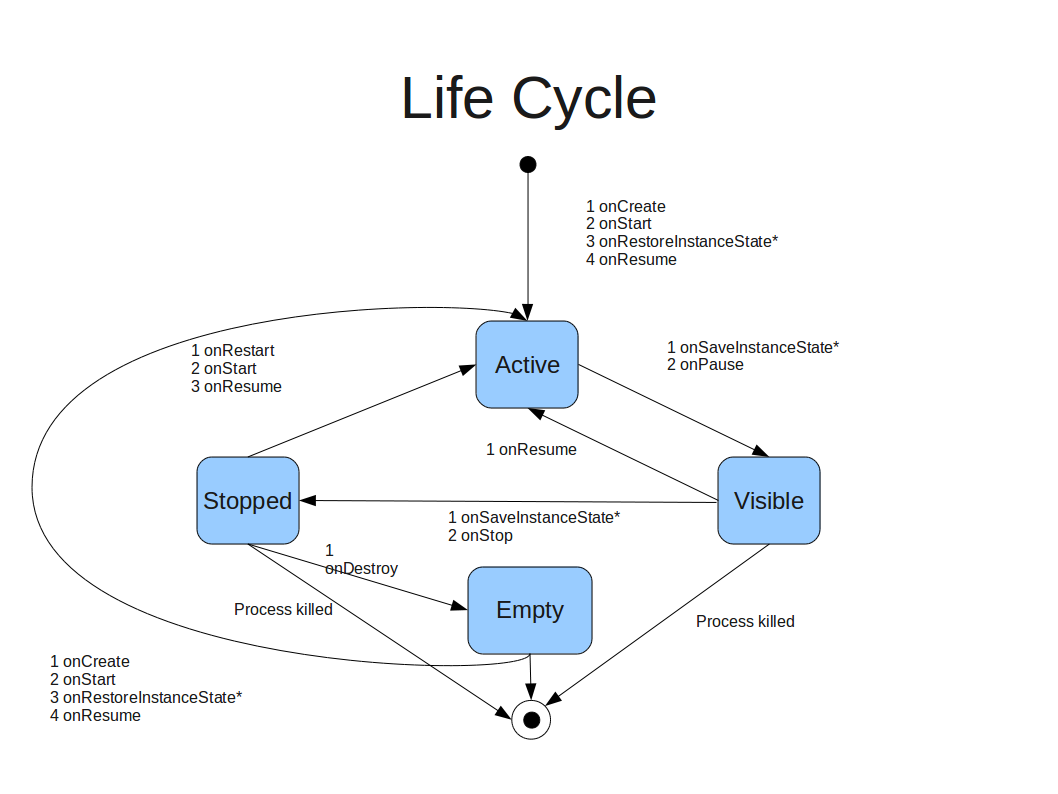
\includegraphics[width=1\textwidth]{imgs/ActivityLifeCycle.jpg}
\captionof{figure}{Rappresentazione ciclo di vita di un Activity}\label{activity_cycle_img}%
\end{center}

Come possiamo notare nella figura \ref{activity_cycle_img}, un ciclo di vita non è altro che una serie di stati attraverso i quali l'Activity passa.
I passaggi tra i diversi stati vengono notificati tramite una callback (metodo) invocata dal sistema.

Quando un activity viene mandata in esecuzione, vengono necessariamente invocati 3 metodi:
onCreate(): l'activity viene creata, e il programmatore dovrà definire le configurazione di base e il layout.

onStart(): l'activity diventa visibile, ed è il momento in cui i servizi e le funzionalità vengono attivate per fornire informazioni all'utente.

onResume(): l'activity diventa la destinazione di tutti gli input dell'utente.



\section{Sketch codice}
Lorem ipsum

\clearpage{\pagestyle{empty}\cleardoublepage}